\section{Sheet Books: Identity and Reading Order}
\label{sec:sheetbooks}

\plain{In brief: this stage answers two questions and deliberately leaves a third alone. Which pieces of the prediction are one sheet? In what order are those sheets read as one unrolls the scroll? It does \emph{not} answer where each sheet lands on the page --- that is Section~\ref{sec:quadribbon} --- and, crucially, it never glues two sheets together in order to make its own answer tidier.}

The natural temptation, once one has a mesh, is to treat each connected component as the unit of identity and assign it an integer wrap. That is what a previous version of this system did, and Section~\ref{sec:deadends} reports how it failed. The difficulty is that mesh connectivity is a statement about geometry, not about papyrus: two pieces of one sheet separated by a hole are disconnected, and two different wraps joined by one fusion are connected. Identity has to be established from evidence that can distinguish the two.

We therefore separate three questions that were previously entangled. Which prediction cells constitute one locally coherent sheet? What winding relation is supported between two such sheets? And how should the accepted geometry be parameterized metrically? A \emph{sheet book} answers the first two without fusing components. A \emph{quad ribbon} answers the third without revising their physical identity.

\subsection{From Slice Skeletons to Sheets}
\label{sec:sheets}

The tracer processes the completed prediction as axial shards of full in-plane slices. On each slice it extracts a pruned skeleton, decomposes it into branch-safe curves, and associates curves between neighbouring planes into \emph{material tracks}.

\paragraph{The in-plane fusion cut.} A single traced curve is not automatically one sheet. A path may follow one wrap, cross a prediction fusion, and continue along another wrap while remaining, throughout, one connected curve --- and every geometric property of that curve is unremarkable. The fusion cut detects the case \emph{along the curve} rather than at a point: samples are classified by whether they lie closer to their own bootstrap track or to another track, and a sustained run of foreign ownership bounded by sustained runs of own ownership triggers a cut. Requiring sustained runs on both sides is what distinguishes a genuine wrap hop from noise at a contact. Association then restarts on the split pieces, so no downstream index ever inherits the fused identity.

\paragraph{Lifting and checking.} For each candidate track, sheet lifting fits a dense single-valued 3-D field over its supported domain and records \emph{direct support} separately from \emph{interpolation} --- a distinction maintained from here to the final pixel.

The ordering of the check is the point. Geometry and support masks are frozen \emph{before} any RAW is sampled; only then is held-out CT consulted, and it must correlate better than a null placement. A track that is too fragmented, shadowed by another surface, normal-flipped, or placed over black CT is rejected. Freezing first is what makes the CT test meaningful: a fit allowed to see RAW would have optimized against exactly the quantity later used to judge it.

The check catches real failures at both extremes --- local bad interpolation, and large prediction phantoms. The $4\times21\times21$ run rejected a 400,000-cell phantom whose fitted geometry landed entirely where the CT was zero; without the check, it would have improved every coverage statistic in the paper.

\begin{table*}[t]
  \caption{Sheet-book ladder. ``Passing material'' is the fraction of evidenced prediction cells carried by sheets whose geometry, support, interpolation, and held-out RAW checks all hold. The criterion is material-weighted rather than count-weighted, because many tiny fragments may fail while the book still carries most of the evidenced papyrus, and many trivial sheets may pass while a major sheet fails.}
  \label{tab:sheet-book}
  \centering
  \small
  \begin{tabular}{@{}lrrrrl@{}}
    \toprule
    Grid & Sheets lifted & Sheets passed & Passing material & Main ordered span & Rejected / order suspended \\
    \midrule
    $4\times5\times5$ & 50 & 49 & 83.7\% & 76 tracks / 17 winds & 1 sheet; 0 ordered tracks \\
    $10\times10\times10$ & 400 & 385 & 74.3\% & 1,058 tracks / 47 winds & 15 sheets; 0 ordered tracks \\
    $4\times21\times21$ & 1,150 & 1,104 & 71.9\% & 2,930 tracks / 102 winds & 46 sheets; 51 tracks \\
    $21\times21\times21$ & 6,500 & 6,188 & 71.4\% & 15,457 tracks / 112 winds & 312 sheets; 174 tracks \\
    \bottomrule
  \end{tabular}
\end{table*}

Table~\ref{tab:sheet-book} shows the ladder after the in-plane fusion cut. Every rung carries more than 70\% of evidenced material, and the shape of the numbers is itself informative: at the largest rung, 6,188 of 6,500 lifted sheets pass, yet the single largest sheet carries only 0.15\% of the material and reaching 70\% of it requires 5,493 tracks. The evidence at full scale is genuinely fragmented. We record that rather than concealing it behind a monolithic fused surface, because a fused surface would have had to invent precisely the connections the fragmentation reports as missing.

\subsection{Winding Assembly Without Geometric Fusion}
\label{sec:winding}

\plain{In brief: accepted sheets still need a reading order --- which is the outer neighbour of which. We measure that from how far apart two sheets sit radially, in units of the \emph{local} spacing, and accept a relation only when it is close to a whole number of turns.}

This section reports book-level order on traced prediction tracks. Section~\ref{sec:prob-winding} addresses the complementary mesh-level problem: fragmented ball-pivoted components receive generalized-winding unary evidence and are optimized jointly as an MRF. The latter does not replace the scale ladder below, and the ladder does not test the new absolute cue.

For two tracks that coexist on sampled planes, we measure their signed separation along the local umbilicus ray and normalize it by the pair's local median inter-wrap spacing. An edge is admitted only when the resulting offset lies within 0.25 turns of an integer; ambiguous offsets contribute no edge.

Using \emph{local} spacing is essential rather than a refinement. Adopting one global 9.5-voxel pitch mislabelled physically separated 12--16-voxel delaminations as two turns rather than one --- the sheet had split, widening the local gap, and a global constant read that widening as an extra wrap. Pitch is a property of a neighbourhood, and treating it as a constant of the scroll manufactures winding errors in exactly the damaged regions where they are hardest to notice.

\paragraph{Composing the relations.} The accepted integer relations form a weighted graph, and it will generally contain cycles that do not close. A Kruskal-style \emph{maximum-support forest} establishes the initial frame, so that when a cycle disagrees, responsibility falls on its weakest-supported edge rather than on an arbitrary one.

A forest alone is not enough, because a single wrong forest edge displaces an entire subtree by a constant offset and no local check can see it: every relation inside the subtree remains perfectly satisfied. We therefore evaluate small integer \emph{subtree shifts}, ranked by the conflicted evidence mass crossing each forest cut, and accept a shift only on a strict reduction in crossing conflict weight. This is loop closure: the cycle-closing relations that the forest discarded are precisely the ones that can detect a globally displaced subtree, and using them is what turns a spanning structure into a checked one.

\paragraph{Quarantine.} If a few tracks remain inconsistent with most of their neighbourhood, we suspend those tracks' \emph{order relations} while retaining their geometry. We do not discard the geometry, and we do not dissolve the component. The reasoning is simple: a contradictory triangle of relations cannot be made consistent by silently deleting one edge and calling the remainder an order. Quarantine is capped at 5\% of a component, and it removes only a claim about reading position --- never papyrus.

\paragraph{Results.} The ordered fraction is 100\% on $4\times5\times5$ and $10\times10\times10$, 98.9\% on $4\times21\times21$, and 99.3\% of assigned material on $21\times21\times21$. On the largest rung, collection covers 95.9 million sampled points; 23,900 accepted winding edges arise from 154,545 candidates, 25 subtree repairs are applied, and 174 tracks (1.1\% of the ordered component) have their order suspended. The median snap residual is 0.12 turns, comfortably inside the 0.25-turn admission bound. Geometry remains separate throughout: a winding edge states an order relation and never welds two tracks.

\begin{figure*}[t]
  \centering
  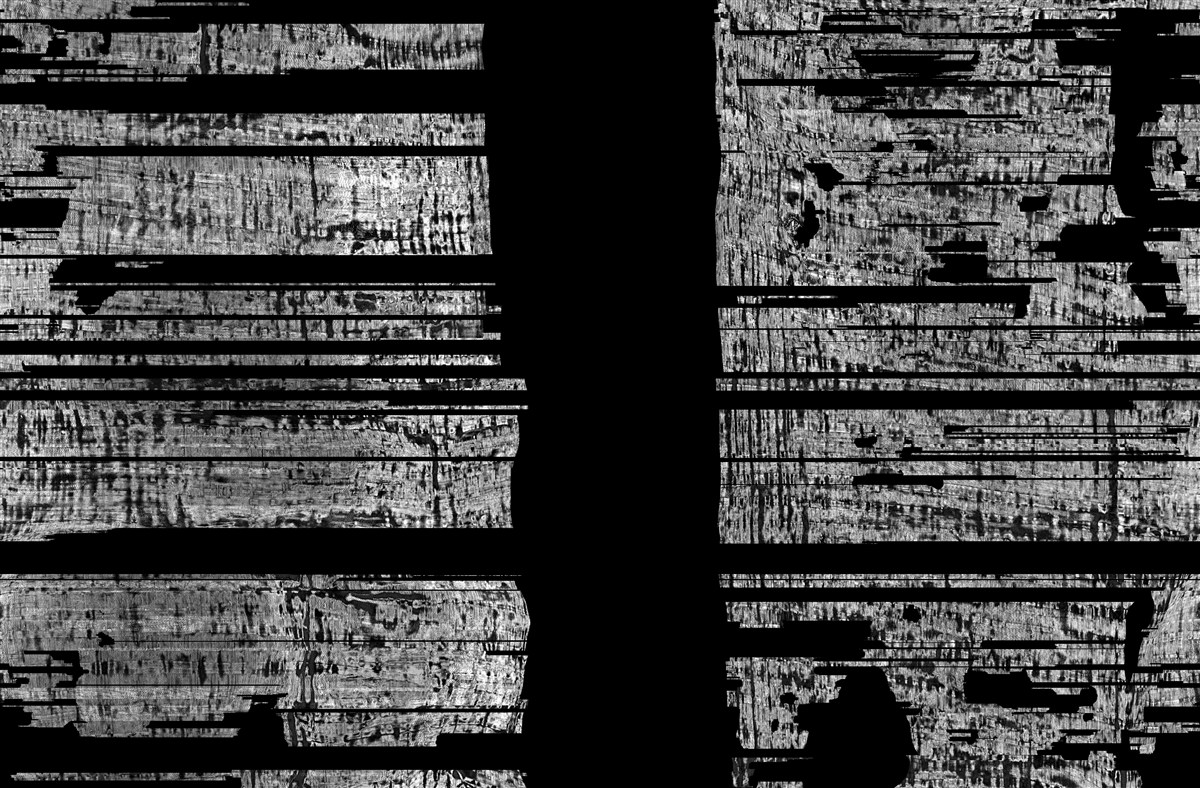
\includegraphics[width=0.80\linewidth]{figures/sheetbook_wind50_preview.jpg}
  \caption{One $21\times21\times21$ winding page assembled from the sheet book. Horizontal fragments are texture-bearing track contributions placed in the inferred reading frame; black gutters and holes remain wherever the book has no accepted track. This is one winding view, and deliberately not a claim of complete page coverage --- the visible gaps are the fragmentation reported in Table~\ref{tab:sheet-book}, shown rather than filled.}
  \Description{A grayscale page-like image containing many horizontal papyrus fragments arranged in two broad columns, with explicit black gaps between unsupported regions.}
  \label{fig:sheetbook-page}
\end{figure*}

The result is an ordered book, not yet a complete solid page. Radial order is established because it is measurable --- a signed separation against a local pitch. Same-wrap continuation across a large unsupported arc has no comparable local measurement, and until it does, a missing track remains a hole in Fig.~\ref{fig:sheetbook-page}.
